%==============================================================================
% ERU Symposium --- Extended Abstract
%
% Formatting follows "1. ERUS Extended-Abstract_Template.docx":
%   A4 paper, two-column body, IEEE conference style, two pages including
%   references. No separate Abstract block (keywords follow the author block).
%
% Compile:  pdflatex extended_abstract_v3.tex   (twice, for references)
%==============================================================================
\documentclass[conference,a4paper,10pt]{IEEEtran}
\IEEEoverridecommandlockouts

\usepackage[a4paper,top=0.75in,bottom=1.0in,left=0.63in,right=0.63in,
            columnsep=0.25in]{geometry}
\usepackage[T1]{fontenc}
\usepackage[utf8]{inputenc}
\usepackage{cite}
\usepackage{amsmath,amssymb}
\usepackage{graphicx}
\usepackage{booktabs}
\usepackage{textcomp}
\usepackage{tikz}
\usetikzlibrary{positioning,arrows.meta}

\raggedbottom

\begin{document}

\title{Inspection-Aware Viewpoint Search for Ground Robots\\
with a Short-Range Fixed Camera}

\author{
\IEEEauthorblockN{Hiruna Malavipathirana}
\IEEEauthorblockA{\textit{Department of Computer Science and Engineering} \\
\textit{University of Moratuwa} \\
Moratuwa, Sri Lanka \\
hirunamalavipathirana.333@gmail.com}
}

\maketitle

\begin{IEEEkeywords}
target search, autonomous exploration, viewpoint planning, coverage,
mobile robots, ROS~2
\end{IEEEkeywords}

%==============================================================================
\section{Introduction}
%==============================================================================
A robot that retrieves objects from an unknown room must do two things: map
the room, and point its detector at every patch of floor where a target could
lie. On a low-cost ground robot these use very different sensors. A 2D~LiDAR
maps \(360^{\circ}\) out to several metres, but its scan plane passes above
small floor-level targets. The RGB-D camera that detects them sees only a
\(57^{\circ}\) forward cone, and only from about \(0.5\) to \(1.0\,\mathrm{m}\):
a single look covers roughly \(0.5\,\mathrm{m}^2\) of floor.

Target-search planners exist, but for platforms that aim the camera cheaply:
a yawing drone~\cite{starsearcher} or an arm~\cite{heats}, with 2--4\,m of
recognition range. On a ground robot with a fixed camera the whole body must
turn to look, turning is slow, and each stop is expensive. Which way to
\emph{inspect} (drive lawnmower rows, stop and look once, or stop and turn)
becomes the central design question, and it has not been studied on real
hardware.

We propose an inspection-aware search framework for this setting.
Its contributions are:
(i)~an inspection map that counts floor as seen only inside the camera's real
footprint;
(ii)~viewpoints that carry a \emph{turn range}, choosing where to stop and how
far to turn there;
(iii)~a per-patch choice between rows and viewpoints based on \emph{measured}
robot costs; and
(iv)~a hardware comparison against four baselines, with ablations of the
inspection method and of the search order.

%==============================================================================
\section{Related Work}
%==============================================================================
Frontier exploration~\cite{yamauchi} stops when the \emph{mapping} sensor has
seen everything, which says nothing about the detector; coverage path
planning~\cite{galceran} sweeps with a tool of known width but assumes a known
map. Star-Searcher~\cite{starsearcher} and HEATS~\cite{heats} track which
occupied voxels the camera has inspected and score viewpoints by a weighted sum
of exploration and inspection gain; HEATS adds region-by-region ordering. Both
show that exploration planners whose sensing range exceeds the recognition
distance miss targets (68.8--95\% completeness~\cite{starsearcher}), and fixing
a manipulator's camera cut region coverage from 82.6\% to 50.2\%~\cite{naazare}.
Gao et al.~\cite{gao} avoid camera coverage by proposing objects from 3D LiDAR
clusters, which fails for targets below a 2D scan plane. None of these choose
\emph{how} to inspect, because their cameras can be aimed freely.

%==============================================================================
\section{Method}
%==============================================================================

\begin{figure}[t]
\centering
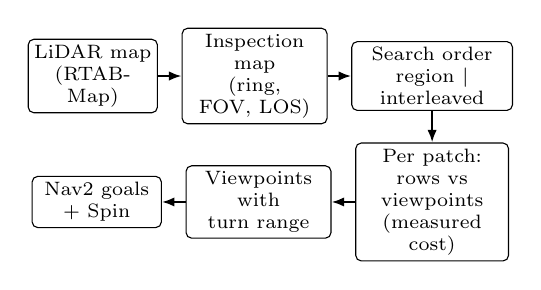
\begin{tikzpicture}[
  box/.style={draw, rounded corners=2pt, align=center, font=\scriptsize,
              minimum height=6.5mm, inner sep=2pt},
  arr/.style={-{Latex[length=1.6mm]}, thick}]
\node[box, text width=15mm] (map) {LiDAR map\\(RTAB-Map)};
\node[box, text width=17mm, right=3mm of map] (insp) {Inspection map\\(ring, FOV, LOS)};
\node[box, text width=19mm, right=3mm of insp] (order) {Search order\\region \(|\)
  interleaved};
\node[box, text width=18mm, below=4mm of order] (choice) {Per patch:\\rows vs viewpoints\\(measured cost)};
\node[box, text width=17mm, left=3mm of choice] (vp) {Viewpoints with\\turn range};
\node[box, text width=15mm, left=3mm of vp] (nav) {Nav2 goals\\+ Spin};
\draw[arr] (map) -- (insp); \draw[arr] (insp) -- (order);
\draw[arr] (order) -- (choice); \draw[arr] (choice) -- (vp);
\draw[arr] (vp) -- (nav);
\end{tikzpicture}
\caption{Framework overview. Only the search order differs between the two
variants we evaluate; everything else is shared.}
\label{fig:overview}
\end{figure}

\subsection{Platform}
A Kobuki base carries a Kinect~v1 (\(57^{\circ}\) FOV, 0.19\,m high), an
RPLIDAR~C1 and a Jetson Orin Nano running ROS~2 Jazzy, RTAB-Map~\cite{rtabmap}
and Nav2~\cite{nav2}. A YOLOv8n model detects the cubes (Fig.~\ref{fig:overview}).

\subsection{Inspection Map}
A floor cell counts as \emph{seen} when it lies in the camera's annulus sector
(\(0.48\)--\(1.0\,\mathrm{m}\), \(\pm 28.5^{\circ}\)) with an unobstructed line of
sight. The inner radius is where the floor enters the image of a level camera;
counting it, as a plain cone does, overstates coverage.

\subsection{Viewpoints with a Turn Range}
Candidates are sampled every 0.25\,m on free floor that is clear enough to turn
in. From each, the visible unseen cells are binned by bearing, so a look that
starts at heading \(\psi\) and turns through span \(s\) covers the bins in
\([\psi-\tfrac{f}{2},\,\psi+s+\tfrac{f}{2}]\), where \(f\) is the FOV. Span
\(s\in\{0,60,\dots,303^{\circ}\}\) runs from one look to a full spin. Each
\((\text{position},\psi,s)\) is scored as area seen per second:
\begin{equation}
J=\frac{A_{\text{new}}(\psi,s)}{t_{\text{travel}}+t_{\text{stop}}+
|\Delta\psi|/\omega+s/\omega}.
\end{equation}
The choice between one look and a spin therefore falls out of one score.

\subsection{Choosing Rows or Viewpoints}
For each unseen patch the planner estimates both methods and uses the faster.
Row time sums fitted leg costs; viewpoint time comes from simulating the
viewpoint planner until 90\% of the patch is seen. The costs were fitted to 129
legs driven on the robot: a row leg costs about \(31\,\mathrm{s}+3.9\,\mathrm{s/m}\)
(52\% of row legs succeeded), a drive to a viewpoint about
\(9.8\,\mathrm{s}+3.4\,\mathrm{s/m}\) (84\% succeeded). An earlier rule based on
patch size sent a whole room to rows and never reached a viewpoint.

\subsection{Search Order}
\emph{Region}: rooms are split at gaps under 1\,m and L-shaped spaces at their
inside corner; the robot explores one region, inspects it until 90\% is seen or
no viewpoint is worth a stop, then moves to the nearest unfinished region.
\emph{Interleaved}: the robot explores the whole map and starts an inspection
round whenever 3\,m\(^2\) of new unseen floor has appeared.

%==============================================================================
\section{Experiments}
%==============================================================================
All runs used the real robot in one furnished, L-shaped lab (about 59\,m\(^2\) of
floor) from a fixed start and HOME, with 6 cubes in fixed places: 4 in the lab
and 2 in an adjoining room that no method reached within the time limit. Each
configuration ran a 15-minute full mission: search, capture, and delivery to
HOME. Baselines:
\textbf{B}, explore then sweep rows;
\textbf{C}, interleaved rows;
\textbf{D}, HEATS-style~\cite{heats} (region order, one look per stop,
0.2/0.8 blended gain);
\textbf{E}, camera-range greedy exploration, as the FUEL control
in~\cite{starsearcher}. Coverage is floor seen against a fixed 59.2\,m\(^2\); AUC
is the mean coverage over the 15\,min. Cubes are counted once each: a delivered
cube that was picked up again at HOME is not counted twice.

\begin{table}[t]
\caption{Full mission, 15\,min: cubes delivered to HOME (of 4 reachable),
time of the 4th delivery, floor seen and coverage AUC.}
\label{tab:bench}
\centering
\setlength{\tabcolsep}{3pt}
\begin{tabular}{lcccc}
\toprule
\textbf{Method} & \textbf{Cubes} & \textbf{4th (s)} &
\textbf{Seen (\%)} & \textbf{AUC (\%)} \\
\midrule
Ours, region order      & 3 & --  & 46.4 & 30.8 \\
Ours, interleaved order & \textbf{4} & \textbf{608} & 49.0 & \textbf{35.2} \\
B (explore, then rows)  & \textbf{4} & 780 & 37.8 & 24.3 \\
C (interleaved rows)    & 2 & --  & 44.6 & 25.8 \\
D (HEATS-style)         & 2 & --  & 40.4 & 21.1 \\
E (greedy, FUEL-style)  & \textbf{4} & 786 & \textbf{51.7} & 29.8 \\
\bottomrule
\end{tabular}
\end{table}

\begin{table}[t]
\caption{Ablations, full mission, 15\,min: inspection method against search
order (cubes delivered; coverage AUC, \%).}
\label{tab:abl}
\centering
\setlength{\tabcolsep}{4pt}
\begin{tabular}{lcccc}
\toprule
& \multicolumn{2}{c}{\textbf{Region order}} & \multicolumn{2}{c}{\textbf{Interleaved}} \\
\cmidrule(lr){2-3}\cmidrule(lr){4-5}
\textbf{Inspection} & Cubes & AUC & Cubes & AUC \\
\midrule
Rows only              & 2 & 23.0 & 2 & 25.8 \\
One look, no turning   & 2 & 29.6 & 4\(^{a}\) & 29.8\(^{a}\) \\
Spin grid (1\,m)       & 4 & 31.5 & -- & -- \\
Viewpoints, turn range & 2 & \textbf{36.4} & 3 & 29.3 \\
Mixed, measured cost   & 3 & 30.8 & 4 & 35.2 \\
\bottomrule
\end{tabular}\\[2pt]
{\scriptsize \(^{a}\)E, greedy one look without regions.}
\end{table}

\subsection{Results}
\textbf{Turning beats rows and single looks.} Under region order, coverage AUC
rose from rows (23.0\%) through one look per stop (29.6\%) and a fixed spin grid
(31.5\%) to viewpoints with a planned turn range (36.4\%), which had seen
20.1\,m\(^2\) after 5\,min against 10.0\,m\(^2\) for rows. The HEATS-style
baseline, one look per stop, reached 21.1\%. Rows fail on this robot for a
physical reason: a straight row that passes near furniture leaves the local
controller with no valid trajectory (all 440 samples rejected), and row legs
stalled or crawled even in open floor. One look per stop pays a full stop for a
0.5\,m\(^2\) view.

\textbf{Measured costs make the per-patch choice work.} In this lab the
measured-cost rule chose viewpoints for every large patch (e.g.\ 702\,s against
1{,}404\,s estimated for rows), while still choosing rows for an open
2\(\times\)12\,m hall. In 5-minute trials, the earlier patch-size rule sent the
whole room to rows and saw 11.0\,m\(^2\); the measured-cost rule saw
19.3\,m\(^2\).

\textbf{Full mission.} The interleaved variant of our method delivered all 4
reachable cubes and was the fastest to do so (608\,s, against 780\,s for B and
786\,s for E), with the highest AUC among the compared methods (35.2\%). Cube
counts also depend on the detector: several cubes were detected but lost while
the robot turned to centre them, which is why the arm with the highest coverage
(region order with viewpoints) delivered 2. No method reversed
while carrying a cube; a delivery that could not continue released the cube and
resumed the search.

\textbf{Search order.} Neither order dominated: region order led with
viewpoints only (AUC 36.4 vs 29.3\%), interleaved order led with the mixed
choice (35.2 vs 30.8\%) and delivered more cubes.

%==============================================================================
\section{Conclusion}
%==============================================================================
For a ground robot whose detector is fixed, forward-facing and short-ranged,
\emph{how} it inspects matters more than when: stopping at chosen viewpoints
and turning through a planned range covered the floor faster than lawnmower rows
and single looks, and a per-patch choice driven by costs measured on the robot
selects the right method automatically. Combined with interleaved exploration,
the framework delivered every reachable target fastest of the methods compared.
Limitations: a single arena, coverage measured on a 2D floor model with a level
camera, and cube counts that depend on detector reliability. Future work: the
search order in multi-room spaces, a time-based rule for leaving a region, and
spins checked against the full robot footprint.

%==============================================================================
\section*{Acknowledgment}
The author thanks supervisor Dr.~Sulochana Sooriyaarachchi for her guidance,
and the Intellisense Lab, Dept.\ of CSE, University of Moratuwa, for
facilities, hardware and funding.

\begin{thebibliography}{00}
\bibitem{starsearcher} Y.~Luo \emph{et al.}, ``Star-Searcher: A complete and
efficient aerial system for autonomous target search in complex unknown
environments,'' \emph{IEEE Robot. Autom. Lett.}, vol.~9, no.~5,
pp.~4329--4336, 2024.
\bibitem{heats} H.~Zhang \emph{et al.}, ``HEATS: A hierarchical framework for
efficient autonomous target search with mobile manipulators,'' in \emph{Proc.
IEEE/RSJ IROS}, 2025, pp.~14371--14378.
\bibitem{yamauchi} B.~Yamauchi, ``A frontier-based approach for autonomous
exploration,'' in \emph{Proc. IEEE CIRA}, 1997, pp.~146--151.
\bibitem{galceran} E.~Galceran and M.~Carreras, ``A survey on coverage path
planning for robotics,'' \emph{Robot. Auton. Syst.}, vol.~61, no.~12,
pp.~1258--1276, 2013.
\bibitem{naazare} M.~Naazare, F.~G.~Rosas, and D.~Schulz, ``Online
next-best-view planner for 3D-exploration and inspection with a mobile
manipulator robot,'' \emph{IEEE Robot. Autom. Lett.}, vol.~7, no.~2,
pp.~3779--3786, 2022.
\bibitem{gao} J.~Gao \emph{et al.}, ``Indoor exploration and simultaneous
trolley collection through task-oriented environment partitioning,'' in
\emph{Proc. IEEE ICRA}, 2024, pp.~14895--14901.
\bibitem{rtabmap} M.~Labb\'{e} and F.~Michaud, ``RTAB-Map as an open-source
lidar and visual simultaneous localization and mapping library for large-scale
and long-term online operation,'' \emph{J. Field Robot.}, vol.~36, no.~2,
pp.~416--446, 2019.
\bibitem{nav2} S.~Macenski \emph{et al.}, ``The Marathon 2: A navigation
system,'' in \emph{Proc. IEEE/RSJ IROS}, 2020, pp.~2718--2725.
\end{thebibliography}

\end{document}
